\chapter{Исследовательская часть}

В данном разделе будут приведены примеры работы программы, а также проведен сравнительный анализ алгоритмов при различных ситуациях на основе полученных данных.

\section{Технические характеристики}

Технические характеристики устройства, на котором выполнялись замеры времени, представлены далее:

\begin{itemize}
	\item операционная система Windows 11 Pro Версия 22H2 (22621.674) \cite{wind};
	\item оперативная память 16 ГБ;
	\item процессор 11th Gen Intel(R) Core(TM) i5-11400, 2.59 ГГц \cite{proc}.
\end{itemize}

При тестировании компьютер был включен в сеть электропитания. Во время замеров времени устройство было нагружено только встроенными приложениями окружения, а также системой тестирования.

\section{Демонстрация работы программы}

На рисунке \ref{img:res} представлен результат работы программы. На экран выводится результат работы программы.
\newpage
%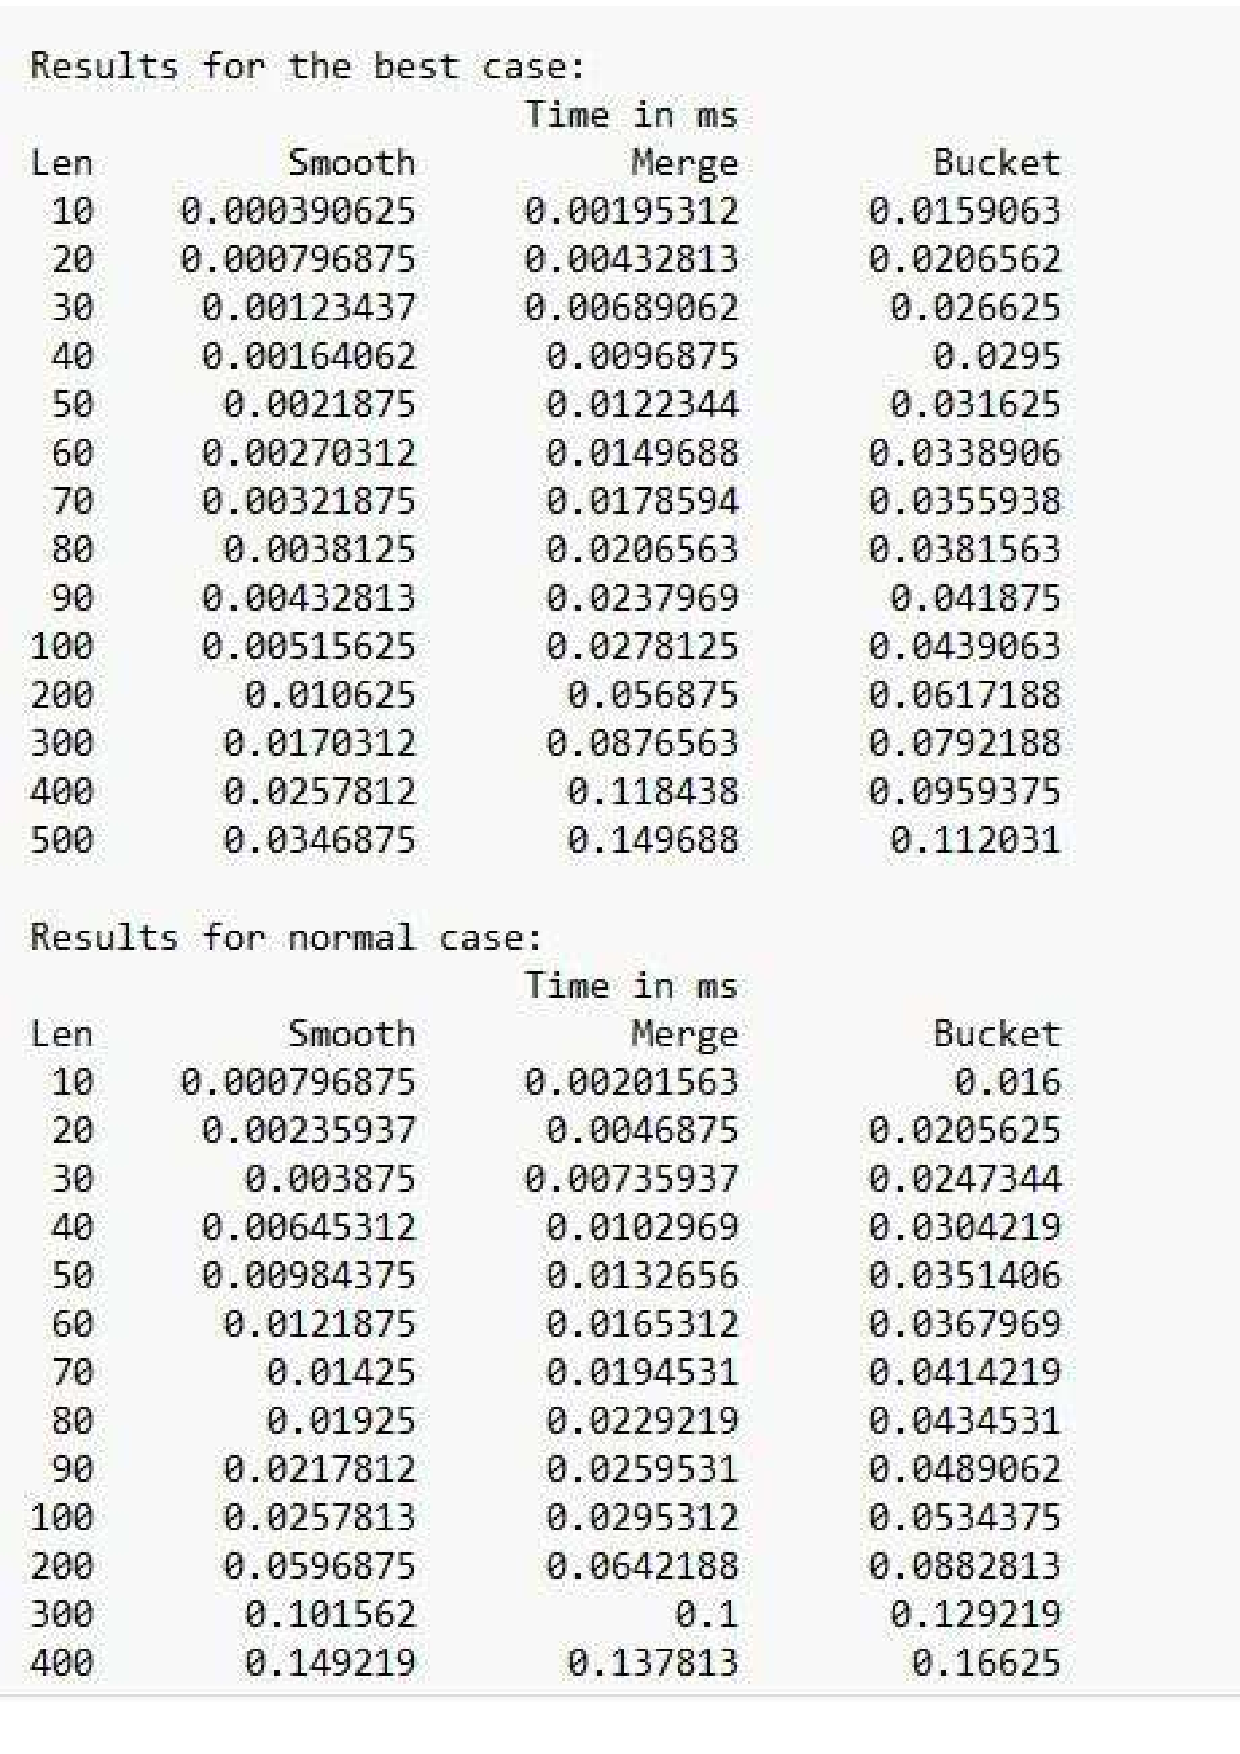
\includepdf[pages=-]{src/screen.pdf}
\begin{center}
	\centering{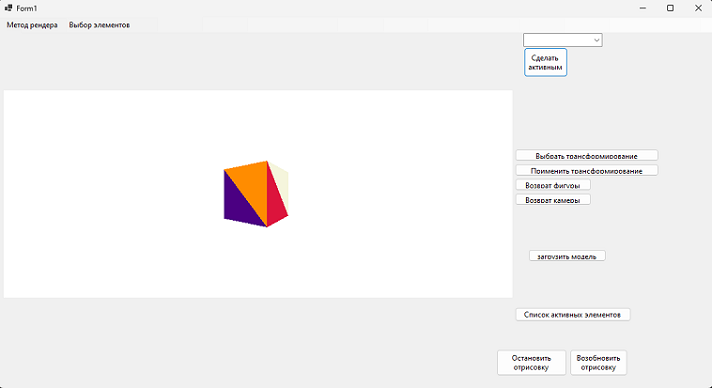
\includegraphics[trim=0.5cm 0 0cm 1cm bb=0 0 758 388]{src/screen}}
	\captionof{figure}{Пример работы программы}
	\label{img:res}
\end{center}

\section{Время выполнения реализаций алгоритмов}

Используются функция замера времени Start() и Stop() из библиотеки $System.Diagnostics$. Для получения времени работы реализаций алгоритма алгоритма используется свойство Elapsed того же класса.

На рисунке \ref{img:graph_sorted},  приведены графические результаты замеров времени работы трассировки лучей для параллельного (при количестве потоков, равном количеству логических ядер ЭВМ, на которой проводились замеры времени, затрачиваемого реализацией трассировки лучей) и последовательного случаев при разной доле заполнения экрана.

\begin{center}
	\centering{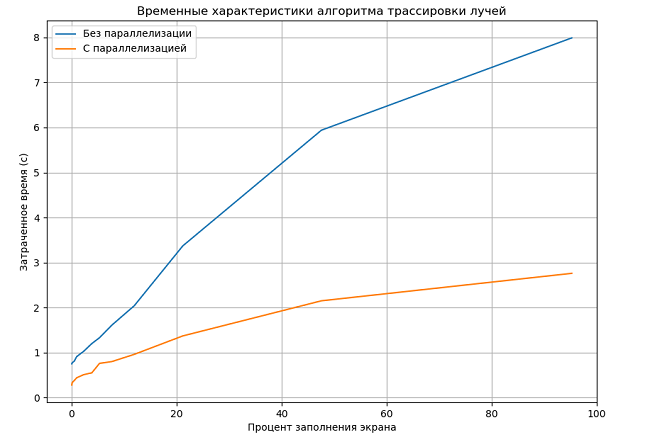
\includegraphics[trim=0 0 0 -5cm bb=0 0 484 650]{src/good}}
	\captionof{figure}{Время работы реализаций алгоритма}
	\label{img:graph_sorted}
\end{center}

\section*{Вывод}
\addcontentsline{toc}{section}{Вывод}
Исходя из полученных результатов, трассировка лучей с параллелизацией окаазалась быстрее в 2.6 раза на большем заполнении экрана и  в 2 раза на меньшем.